\section{准备工作}

\subsection{国际标准大气模型}

因为在计算飞行器飞行性能时,
往往需要大气参数(在各个高度上的温度、密度压强等)值,
才能得到计算结果,
比如升力与阻力的计算中需要用到大气高度上的密度$\rho$与声速$a$。
因此在计算飞行性能前,需要构建一个可用的大气模型。

为了满足飞机的设计与计算,处理和分析飞机的飞行试验数据,
进行飞行性能参数计算等方面的需求,国际民航组织(ICAO)制定了国际标准大气(ISA)
作为为衡量、比较飞机性能的公共的标准。
本文也拟采用该大气模型作为估算飞行性能的标准。

\subsubsection{大气性质}

大气的基本基本状态参量温度$T$、压强$p$和密度$\rho$满足大气状态方程:
\begin{equation}
    \label{大气状态方程}
    p=\rho RT
\end{equation}
上式中$p$单位为$Pa(N/m^2)$,$\rho$单位为$kg/m^3$,$T$单位为开尔文$K$。
$R$为大气的气体常数,通常取为:
\begin{equation}
    R=287.06 (N\cdot m)/(kg\cdot K)
\end{equation}

在计算过程中,大气中的声速也是一个常用的参数指标。
声波是一种微弱的扰动波,在传递过程
中只有压力波(压强)的变化而引起传递介质疏密程度的变化产生的振动,并没
有物质的交换。在飞机的飞行性能分析中大气的声速是用来表征空气压缩性的参
量或尺度。大气中声速取决于大气的温度,声速$c(m/s)$的计算公式为:
\begin{equation}
    \label{声速计算公式}
    c = \sqrt{\gamma RT}
\end{equation}
其中$\gamma$比热比,对于空气而言取为$1.4$。
为带入式\ref{大气状态方程}可得另一个声速计算公式如下:
\begin{equation}
    \label{声速计算公式2}
    c = \sqrt{\gamma\frac{p}{\rho}}
\end{equation}

另外,平静大气的压强$p$随高度$h$的变化规律满足如下流体静力学方程:
\begin{equation}
    \label{流体静力学方程}
    dp = -\rho g dh
\end{equation}
上式中$g$表示重力加速度,单位$m/s^2$,高度为$h$,单位为$m$。

\subsubsection{海平面大气数据}

在各个高度上的大气数据需要选取一个海拔基准,
ISA一般采用海平面参数作为基准。
在海拔为$0$的海平面上,
规定大气参数如下:

\begin{equation}
    \begin{cases}
        \begin{aligned}
            T_0 & = 15^{\circ}C = 288.15K\\
            p_0 & = 1013.25hPa\\
            \rho_0 & = 1.225kg/m^3\\
            c_0 & = 340.294 m/s\\
            g_0 & = 9.80665 m/s^2
        \end{aligned}
    \end{cases}
\end{equation}

需要注意的是,因为飞行器的飞行高度往往在海拔$30km$以内,
在此范围内,
温度、密度、压强和声速参数有较剧烈变化,
而因为$30km$高度相较于地球半径而言是一个小量,
因此在此范围内不考虑重力加速度$g_0$值的变化。

\subsubsection{标准大气模型}

在考虑飞行高度时,
往往将大气划分为两个部分:对流层(troposphere)和平流层(tratosphere)。
一般而言将海拔$0\sim 11km$的高度定义为对流层,
该范围内大气参数变化明显,而平流层定义为$11km\sim 20km$部分,
该范围内大气参数变化较为平缓。

其中温度在对流层内的计算公式为:
\begin{equation}
    T(h) = T_0 - \lambda h\quad h\leq 11km
\end{equation}
上式中$\lambda$为$6.5^{\circ}C/km$,表明海拔每上升$1km$,
气温下降$6.5$摄氏度。
而在平流层内温度近似不变为:
\begin{equation}
    T(h) \approx T(11km) = 216.65K
\end{equation}

带入\ref{流体静力学方程}得到:
\begin{equation}
    \frac{dp}{p} = -\frac{g}{R}\frac{dh}{T(h)}
\end{equation}

于是可以推导得到大气压强$p$的取值:
\begin{equation}
    p(h)=
    \begin{cases}
        \begin{aligned}
            &p_0 \left(  \frac{T_h}{T_0}\right)^{\frac{g_0}{R\lambda}} \quad h\leq 11km\\
            &p_{11} e^{-\frac{g(h - h_{11})}{RT_{11}}} \quad 11km<h \leq 20km
        \end{aligned}
    \end{cases}
\end{equation}
上式中,脚标$0$表示海平面参数,脚标$11$表示参数在对流层顶部$11km$处的取值。

类似地,运用式\ref{大气状态方程}可以计算得到密度的高度分布:
\begin{equation}
    \rho (h)=
    \begin{cases}
        \begin{aligned}
            &\rho_0\left(\frac{T_h}{T_0}\right)^{\frac{g}{R\lambda} - 1} \quad h\leq 11km\\
            & \rho_{11} e^{-\frac{g(h - h_{11})}{RT_{11}}} \quad 11km<h \leq 20km
        \end{aligned}
    \end{cases}
\end{equation}

而在高度$h$上的声速则可以用式\ref{声速计算公式}计算得到,
上述大气参数分布如下图中展示。

\begin{figure}[H]
    \centering
    \subfloat[$h-T$温度高度分布]{
        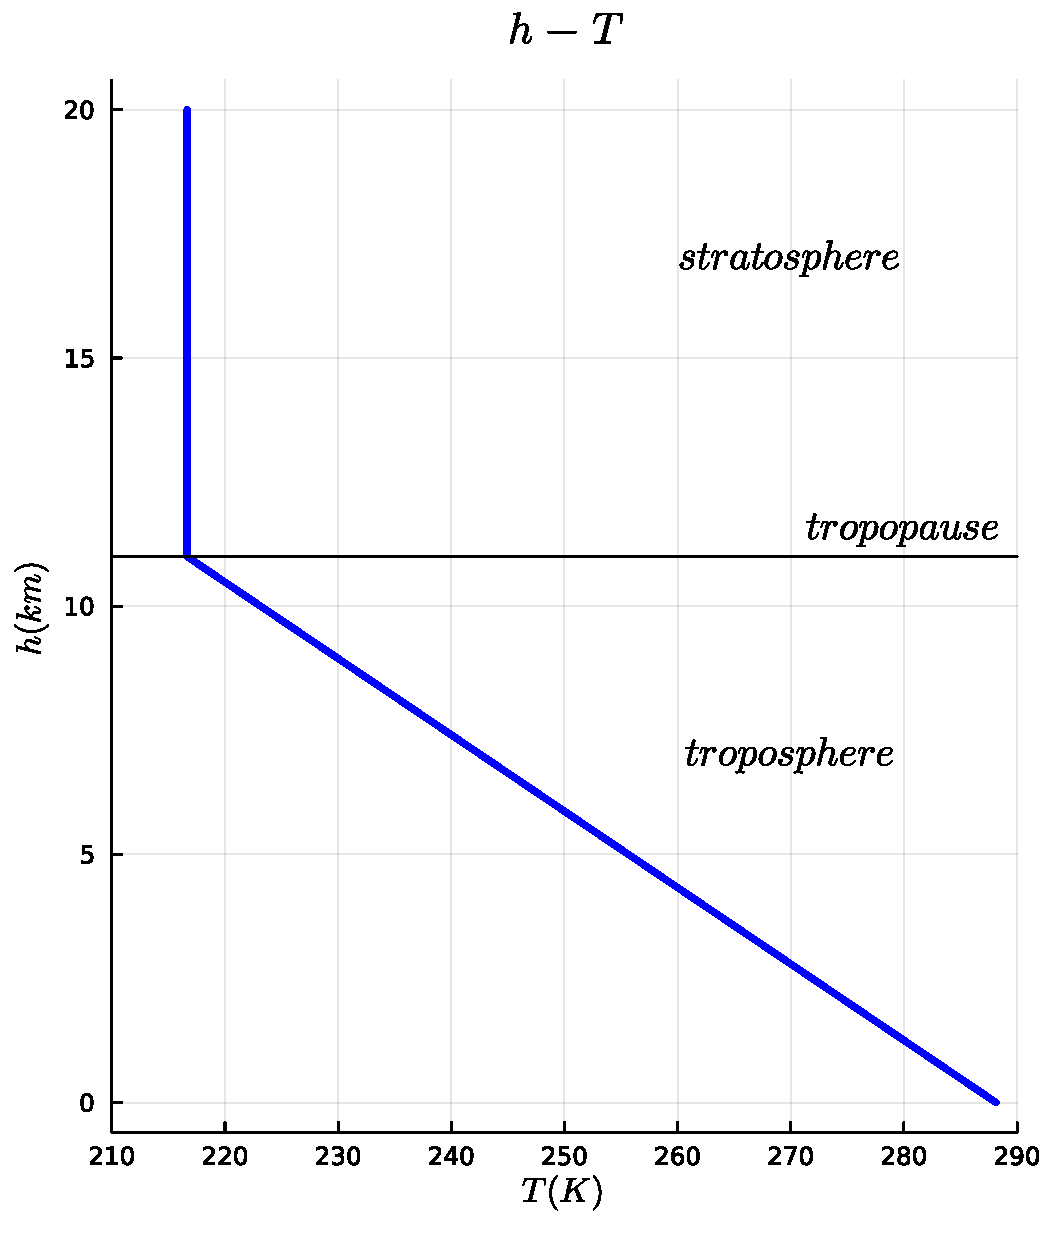
\includegraphics[width=0.4\textwidth]{image/ch2/T_distribution.pdf}
        \label{温度高度分布}
    }
    \subfloat[$h-p$压强高度分布]{
        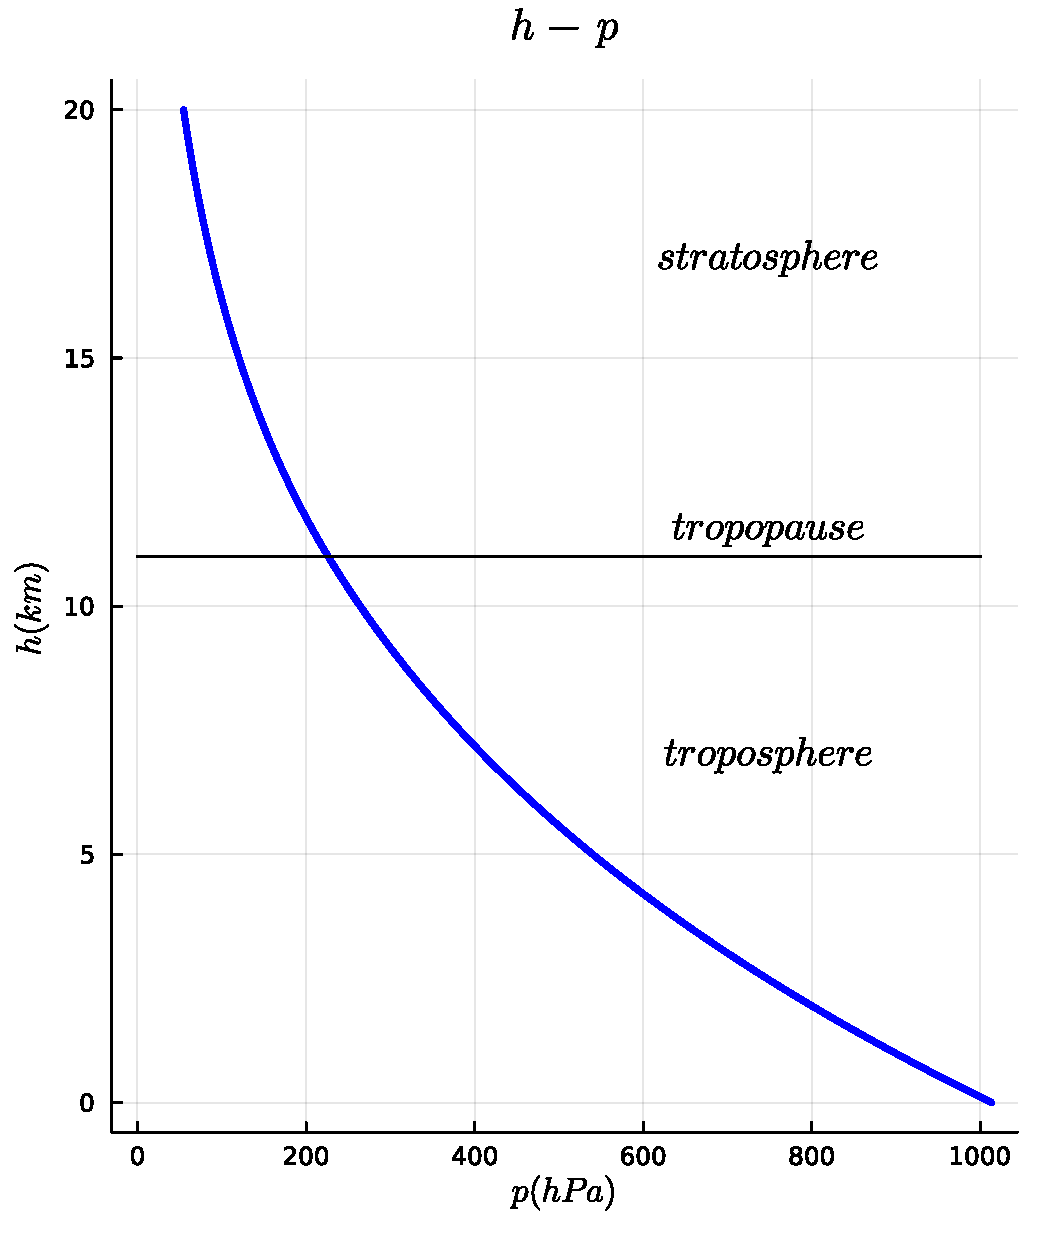
\includegraphics[width=0.4\textwidth]{image/ch2/p_distribution.pdf}
        \label{压强高度分布}
    }
    \quad
    \subfloat[$h-\rho$密度高度分布]{
        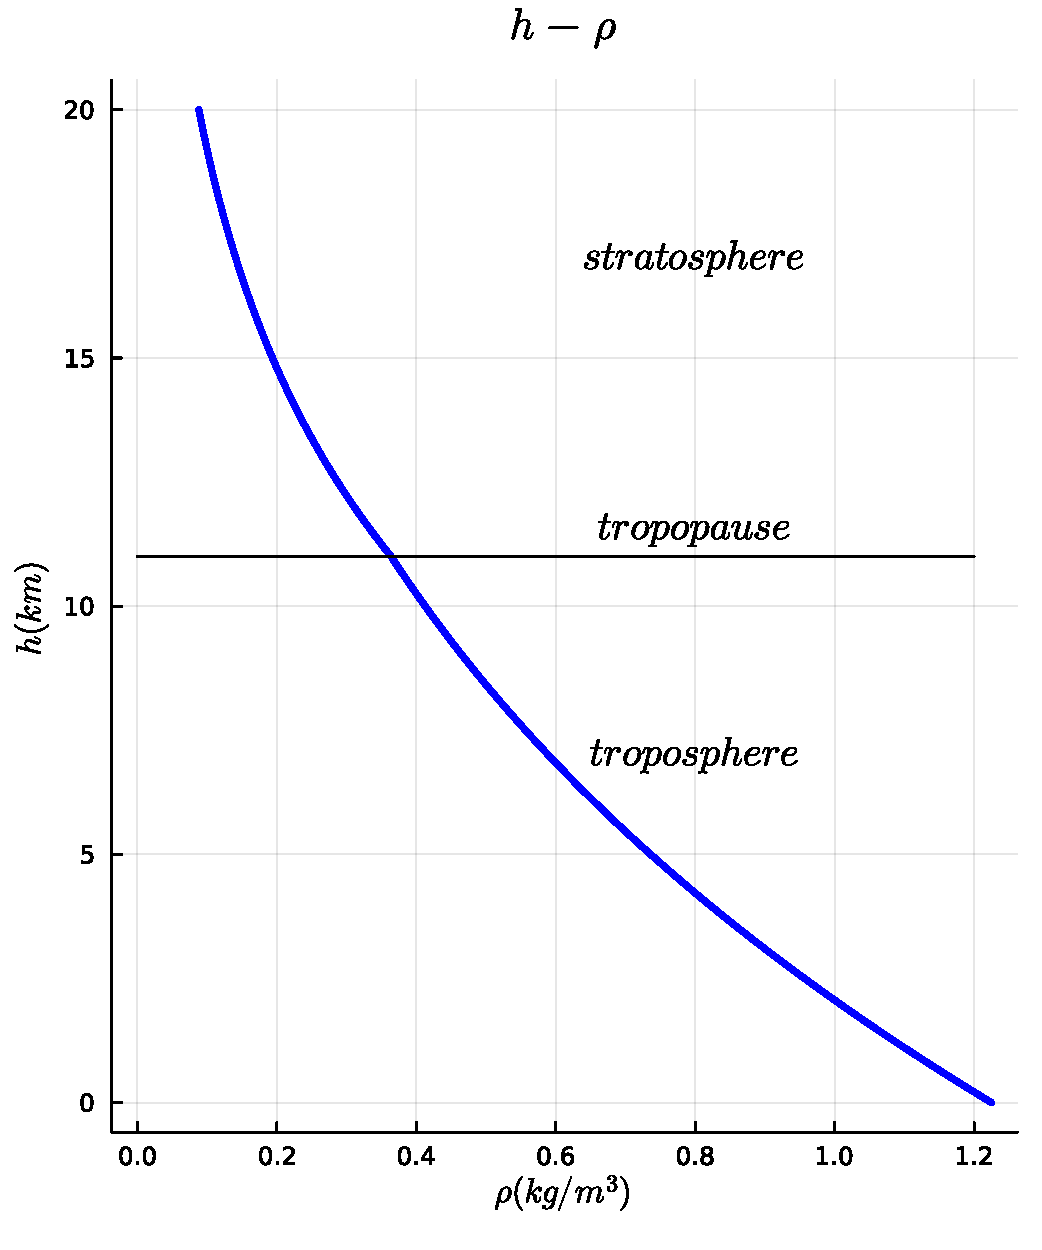
\includegraphics[width=0.4\textwidth]{image/ch2/rho_distribution.pdf}
        \label{密度高度分布}
    }
    \subfloat[$h-c$声速高度分布]{
        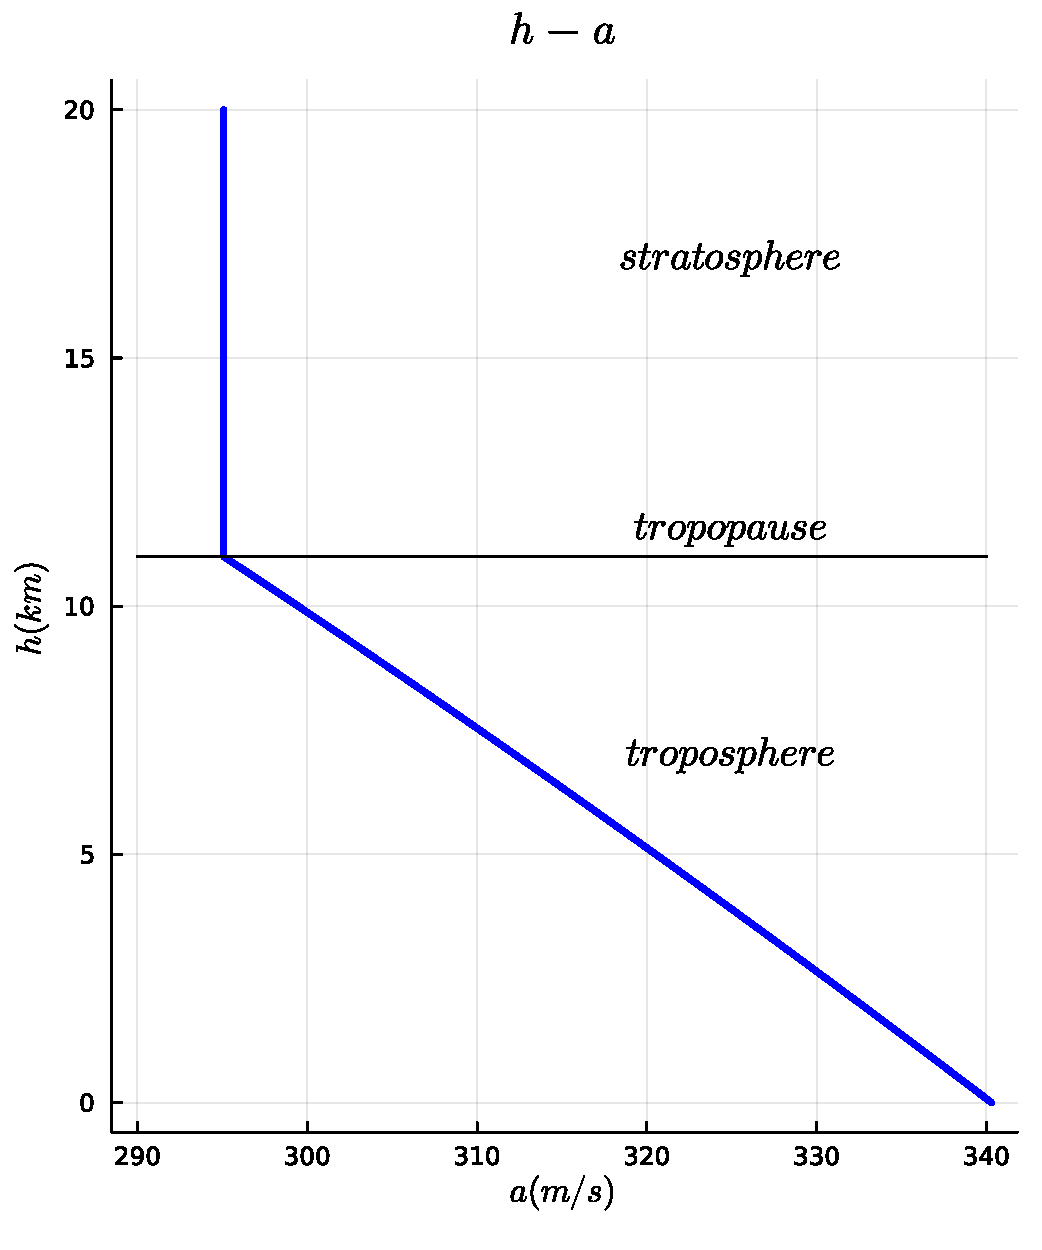
\includegraphics[width=0.4\textwidth]{image/ch2/a_distribution.pdf}
        \label{声速高度分布}
    }
\end{figure}







\subsection{拟合原理及方法}

因为在本次作业中,
往往需要涉及到曲线值的拟合,
如参数$C_L-C_D$之间极曲线关系,
其极曲线参数$A$与$C_{D0}$是由拟合得到的,
因此在准备工作中有必要说明本文采取的方法。

\subsubsection{最小二乘法拟合多项式函数}

现考虑有$M$个离散的采样点$(x_j,y_j)(j=1\sim M)$,
其关系为$f(x)$为一$N$次多项式函数,则可以表达为:
\begin{equation}
    y = f(x) = \sum_{k=0}^N a_k x^k
\end{equation}

考虑每一个采样点上的残差:
\begin{equation}
    r_j = y_j - f(x)_j = y_j - \sum_{k=0}^N a_k x_j^k
\end{equation}

最小二乘法要让上述每个点上残差的平方和最小,为此要求:
\begin{equation}
    R =\sum_{j=1}^M r_j^2 =\sum_{j=1}^M \left( y_j - \sum_{k=0}^N a_k x_j^k\right)^2
\end{equation}
中$R$取为最小值。

在$R$取最小值时,可以给出如下$N$个方程:
\begin{equation}
    \frac{\partial R}{\partial a_k} = 0 \quad k=0\sim N
\end{equation}
即:
\begin{equation}
    \sum_{j=1}^M x_{j}^k y_j = \sum_{j=1}^M x_j^k \sum_{k=0}^N x_j^k a_k\quad k=0\sim N
\end{equation}
上式可以改写成矩阵乘法的形式:
\begin{equation}
    \begin{bmatrix}
        \sum_{j=1}^M  y_j\\
        \sum_{j=1}^M x_{j}^1 y_j\\
        \vdots\\
        \sum_{j=1}^M x_{j}^N y_j
    \end{bmatrix}_{N+1}
    =
    \begin{bmatrix}
        M & \sum_{j=1}^M x_{j}^1 & \cdots & \sum_{j=1}^M x_{j}^N \\
        \sum_{j=1}^M x_{j}^1 & \sum_{j=1}^M x_{j}^2 & \cdots & \sum_{j=1}^M x_{j}^{N+1} \\
        \vdots & \vdots & \ddots & \vdots \\
        \sum_{j=1}^M x_{j}^{N} & \sum_{j=1}^M x_{j}^{N+1} & \cdots & \sum_{j=1}^M x_{j}^{2N}
    \end{bmatrix}_{N+1\times N+1}
    \begin{bmatrix}
        a_0 \\ a_1 \\ \vdots \\ a_N
    \end{bmatrix}_{N+1}
\end{equation}

记符号$Y=[y_1, y_2,\cdots,y_M]^T$,$A=[a_0,a_1,\cdots,a_N]^T$和符号$X$如下有:
\begin{equation}
    X^T Y = X^T X A \quad \leftarrow 
    X=
    \begin{bmatrix}
        1 & x_1 & \cdots & x_1^N\\
        1 & x_2 & \cdot & x_2^N \\
        \vdots & \vdots & \ddots & \vdots \\
        1 & x_M & \cdots & x_M^N
    \end{bmatrix}_{M\times N+1}
\end{equation}

根据上式,可以计算得到最小二乘法拟合下的参数估计值:
\begin{equation}
    \label{最小二乘法}
    A = (X^T X)^{-1} X^T Y
\end{equation}

\subsubsection{拟合方法}

在julia语言中,Curve\_Fit.jl库是采用最小二乘法进行曲线拟合的一个外部库,
其可以用简短的语言进行曲线参数拟合。
但因本次作业的$C_L-C_D$极曲线参数拟合以及$C_{l.\alpha}-C_L$线性回归拟合
均属于比较简单的最小二乘法拟合,
因此本次作业不再依赖外部库实现。





\subsection{插值原理及方法}

因为在本次作业中,
往往需要根据离散点进行插值,
而线性插值因为难以表现离散点的变化趋势,
因此本文采用样条插值(spline)进行内部插值。

\subsubsection{三次样条插值原理}

同样考虑一系列离散的采样点$(x_j,y_j)(j=1\sim N)$,
记区间长度$h_j = x_{j+1} - x_{j}$,
$x_j$节点上的二阶导数值为$M_j$,于是可以得到区间$[x_j,x_{j+1}]$上的样条插值函数$S(x)$的二阶导数:
\begin{equation}
    S^{\prime\prime}(x) = M_j + \frac{1}{h_j}(M_{j+1} - M_j)(x - x_j)\quad x\in [x_j,x_{j+1}]
\end{equation}

对上式积分两次,利用$S(x_j) = y_j$和$S(x_{j+1}) = y_{j+1}$可以计算得到:
\begin{equation}
    \label{样条插值}
    \begin{aligned}
        S(x)=& M_J \frac{(x_j+1 - x)^3}{6h_j} + M_{j+1} \frac{(x-x_j)^3}{6h_j}\\
        & +\left( y_j - \frac{1}{6}M_j h_j^2 \right) \frac{x_j+1 - x}{h_j}
        +
        \left( y_{j+1} - \frac{1}{6}M_{j+1}h_j^2\right)\frac{x-x_j}{h_j}
    \end{aligned}
\end{equation}

为使得样条插值函数$S(x)$在整个插值区域上二阶连续,
因为原函数连续已经保证,二阶导连续也已经保证,只需要满足
$S^{\prime}(x_j^+) =S^{\prime}(x_j^-) $:
\begin{equation}
    f[x_j, x_{j+1}] + \left(\frac{1}{6}M_j + \frac{1}{3}M_{j+1}\right)h_j
    =
    f[x_{j-1}, x_j] + \left(\frac{1}{6}M_{j-1} + \frac{1}{3}M_j\right)h_{j-1}
\end{equation}

引入如下记号:
\begin{equation}
    \mu_j = \frac{h_{j-1}}{h_{j-1}+h_j}\quad \lambda_j = 1 - \mu_j
    \quad
    d_j = 6f[x_{j-1}, x_{j}, x_{j+1}]
\end{equation}

可以得到矩阵形式(这往往需要给定边界条件):
\begin{equation}
    \begin{bmatrix}
        2 & 1 & 0 & \cdots & 0\\
        \mu_2 & 2 & \lambda_2 & \cdots & 0\\
        0 & \ddots & \ddots & \ddots &0\\
        0 & \cdots & \mu_{N-1} & 2 & \lambda_{N-1}\\
        0 & \cdots & 0 & 1 & 2
    \end{bmatrix}
    \begin{bmatrix}
        M_1 \\ M_2 \\ \vdots \\ M_{N-1} \\ M_N
    \end{bmatrix}
    =
    \begin{bmatrix}
        d_1 \\ d_2 \\ \vdots \\ d_{N-1} \\ d_{N}
    \end{bmatrix}
\end{equation}

因为对于一系列散点,其边界条件无法给定,
所以在实际操作中,
往往会对$1\sim 2$点用局部线性插值,$N-1\sim N$点也用局部线性插值,
再对剩余的内部节点利用上式进行三次样条插值。

\subsubsection{样条插值方法}

因为本次作业的原始数据均为离散点,
所以在计算性能过程中为了得到连续变化的趋势需要进行样条插值。
因样条插值的过程较为复杂,
且没必要特地去实现一个这样功能的函数,
因此本文直接使用julia语言中的Dierckx.jl库进行数据插值处理。